% !TeX spellcheck = en_US
% !TeX encoding = utf8
% !TeX program = xelatex
% !BIB program = bibtex
% \documentclass[mathserif,compress,12pt]{ctexbeamer}
\documentclass[12pt,notes,mathserif]{beamer}
% \documentclass[draft]{beamer}	
\usetheme{Singapore}
% \usetheme{Hannover}
%\usepackage{pgfpages}
%\setbeameroption{show notes on second screen}

\usepackage[british]{babel}
\usepackage{graphicx,hyperref,url}
% \usepackage{ru}
\usepackage{mmstyles,bm,ulem}

\usepackage{listings}
\usefonttheme[onlymath]{serif}
\usepackage{fontspec}
\usepackage{xeCJK}
% \setCJKfamilyfont{hei}{SimHei}
% \setCJKmainfont[BoldFont=Arial, ItalicFont=Arial]{Arial}
% \pgfdeclareimage[width=\paperwidth,height=\paperheight]{bg}{background}
% \setbeamertemplate{background}{\pgfuseimage{bg}}
%% columns
\newcommand{\begincols}[1]{\begin{columns}{#1}}
\newcommand{\stopcols}{\end{columns}}
% \usepackage[backend=biber]{biblatex}
% \bibliography{./ref.bib}
%\addbibresource{ref.bib}
\usepackage{indentfirst}
\usepackage{longtable}
\usepackage{float}
%\usepackage{picins}
\usepackage{rotating}
\usepackage{subfigure}
\usepackage{tabu}
\usepackage{amsmath}
\usepackage{amssymb}
\usepackage{setspace}
\usepackage{amsfonts}
\usepackage{appendix}
\usepackage{listings}
\usepackage{xcolor}
\usepackage{colortbl}
\usepackage{geometry}
% \setCJKfamilyfont{cjkhwxk}{SimSun}
% \newcommand*{\cjkhwxk}{\CJKfamily{cjkhwxk}}
%\newfontfamily{\consolas}{Consolas}
%\newfontfamily{\monaco}{Monaco}
%\setmonofont[Mapping={}]{Consolas}	%英文引号之类的正常显示,相当于设置英文字体
%\setsansfont{Consolas} %设置英文字体 Monaco, Consolas,  Fantasque Sans Mono
% \setmainfont{Times New Roman}
% \newfontfamily{\consolas}{Times New Roman}
% \newfontfamily{\monaco}{Arial}
% \setCJKmainfont{Times New Roman}
%\setmainfont{MONACO.TTF}
%\setsansfont{MONACO.TTF}
\newcommand{\verylarge}{\fontsize{60pt}{\baselineskip}\selectfont}  
\newcommand{\chuhao}{\fontsize{44.9pt}{\baselineskip}\selectfont}  
\newcommand{\xiaochu}{\fontsize{38.5pt}{\baselineskip}\selectfont}  
\newcommand{\yihao}{\fontsize{27.8pt}{\baselineskip}\selectfont}  
\newcommand{\xiaoyi}{\fontsize{25.7pt}{\baselineskip}\selectfont}  
\newcommand{\erhao}{\fontsize{23.5pt}{\baselineskip}\selectfont}  
\newcommand{\xiaoerhao}{\fontsize{19.3pt}{\baselineskip}\selectfont} 
\newcommand{\sihao}{\fontsize{14pt}{\baselineskip}\selectfont}      % 字号设置  
\newcommand{\xiaosihao}{\fontsize{12pt}{\baselineskip}\selectfont}  % 字号设置  
\newcommand{\wuhao}{\fontsize{10.5pt}{\baselineskip}\selectfont}    % 字号设置  
\newcommand{\xiaowuhao}{\fontsize{9pt}{\baselineskip}\selectfont}   % 字号设置  
\newcommand{\liuhao}{\fontsize{7.875pt}{\baselineskip}\selectfont}  % 字号设置  
\newcommand{\qihao}{\fontsize{5.25pt}{\baselineskip}\selectfont}    % 字号设置 

\graphicspath{{./fig/}}

% \setbeamertemplate{footnote}{%
%   \hangpara{2em}{1}%
%   \makebox[2em][l]{\insertfootnotemark}\footnotesize\insertfootnotetext\par%
% }

\definecolor{cred}{rgb}{0.6,0,0}
\definecolor{cgreen}{rgb}{0.25,0.5,0.35}
\definecolor{cpurple}{rgb}{0.5,0,0.35}
\definecolor{cdocblue}{rgb}{0.25,0.35,0.75}
\definecolor{cdark}{rgb}{0.95,1.0,1.0}
\lstset{
	language=R,
	numbers=left,
	numberstyle=\tiny\color{black},
	keywordstyle=\color{cpurple}\consolas,
	commentstyle=\color{cgreen}\consolas,
	stringstyle=\color{cred}\consolas,
	frame=single,
	escapeinside=``,
	xleftmargin=1em,
	xrightmargin=1em, 
	backgroundcolor=\color{cdark},
	aboveskip=1em,
	breaklines=true,
	tabsize=3
} 

\providecommand{\tightlist}{%
  \setlength{\itemsep}{0pt}\setlength{\parskip}{0pt}}

  
% The title of the presentation:
%  - first a short version which is visible at the bottom of each slide;
%  - second the full title shown on the title slide;
% \title[]{\LARGE CSE 5526: Introduction to Neural Networks}

% Optional: a subtitle to be dispalyed on the title slide
\title{Support Vector Machines (SVMs) \\Part 3: Kernels}

% The author(s) of the presentation:
%  - again first a short version to be displayed at the bottom;
%  - next the full list of authors, which may include contact information;
\author[YingmingLi]{Yingming Li \\ yingming@zju.edu.cn}
% The institute:
%  - to start the name of the university as displayed on the top of each slide
%    this can be adjusted such that you can also create a Dutch version
%  - next the institute information as displayed on the title slide

\institute[DSERC, ZJU]{Data Science \& Engineering Research Center, ZJU}
% Add a date and possibly the name of the event to the slides
%  - again first a short version to be shown at the bottom of each slide
%  - second the full date and event name for the title slide
\date[\today]{\today}

\begin{document}

\AtBeginSection[]
{
	\begin{frame}
		\frametitle{Outline}
		\tableofcontents[currentsection]
	\end{frame}
}

% \AtBeginSubsection[2-]
% {
%    \begin{frame}
%        \frametitle{Outline}
%        \tableofcontents[currentsection]
%    \end{frame}
% }
\begin{frame}[c]
	\titlepage
	\begin{center}
		Adapted from slides provided by Prof. Michael Mandel.
	\end{center}
\end{frame}

% 2
\begin{frame}[c]
\frametitle{Kernels are generalizations of inner products}
\begin{itemize}
\item A kernel is a function of two data points such that
\[
k(x,x')=\phi^T(x)\phi(x')
\]
For some function $\phi(x)$
\item It is therefore symmetric: $k(x,x')=k(x',x)$
\item Can compute $k(x,x')$ from an explicit $\phi(x)$
\item Or prove that $k(x,x')$ corresponds to some $\phi(x)$
\begin{itemize}
\item Never need to actually compute $\phi(x)$
\end{itemize}
\end{itemize}

\end{frame}


% 3
\begin{frame}[c]
\frametitle{SVM as a kernel machine}
\begin{itemize}
\item {\bf Cover's theorem:} A complex classification problem, cast in a high-dimensional space nonlinearly, is more likely to be linearly separable than in the low-dimensional input space

\item SVM for pattern classification
\begin{itemize}
\item Nonlinear mapping of the input space onto a high-dimensional feature space
\item Constructing the optimal hyperplane for the feature space
\end{itemize}

\end{itemize}
\end{frame}

% 4
\begin{frame}[c]
\frametitle{Kernel machine illustration}
\begin{center}
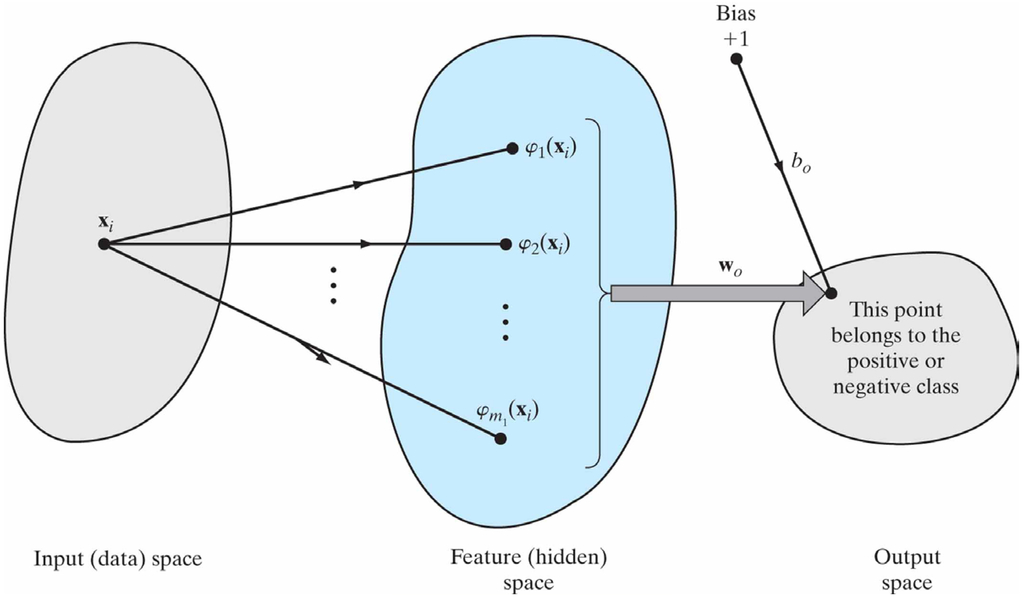
\includegraphics[width=0.7\linewidth]{fig10/lec104.jpg}
\end{center}
\end{frame}

% 5
\begin{frame}[c]
\frametitle{Kernelized SVM looks a lot like an RBF net}
\begin{center}
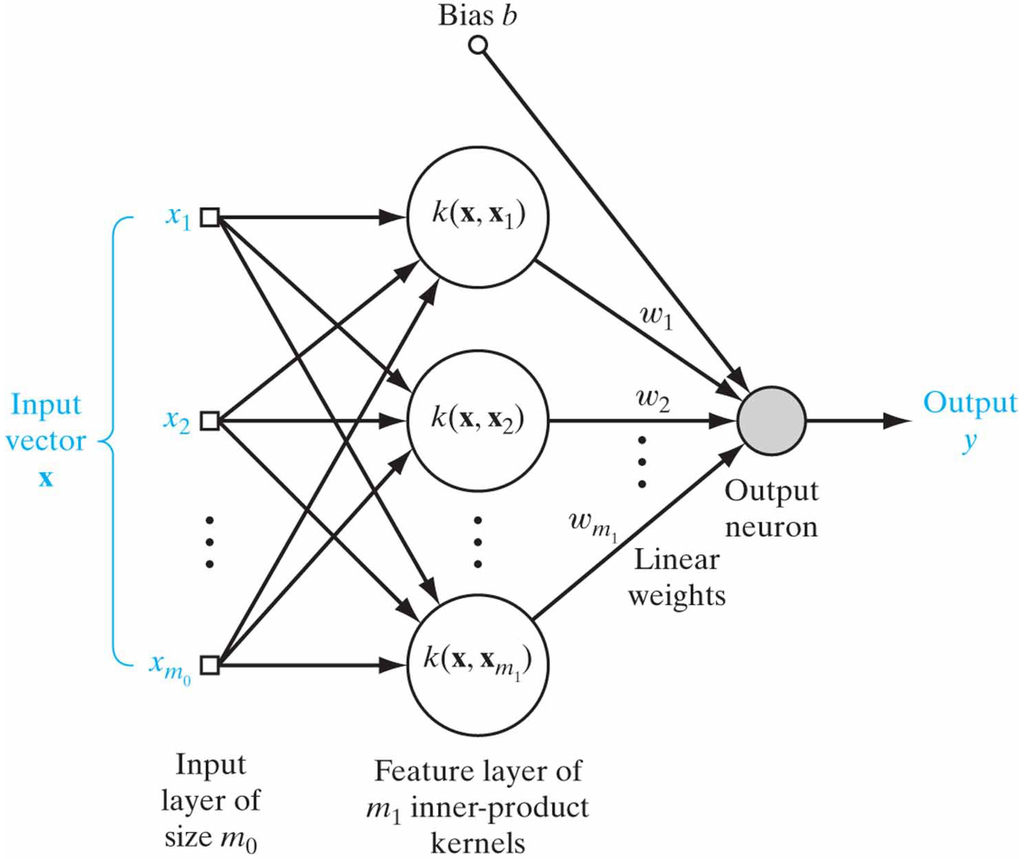
\includegraphics[width=0.7\linewidth]{fig10/lec105.jpg}
\end{center}
\end{frame}

% 6
\begin{frame}[c]
\frametitle{Kernel matrix}
\begin{itemize}
\item The matrix
\[
\mathbf{K}=
\begin{bmatrix}
k(\mathbf{x}_1,\mathbf{x}_1)&\cdots&k(\mathbf{x}_1,\mathbf{x}_N)\\
&\vdots&\\
\cdots&k(\mathbf{x}_i,\mathbf{x}_j)&\cdots\\
&\vdots&\\
k(\mathbf{x}_N,\mathbf{x}_1)&\cdots&k(\mathbf{x}_N,\mathbf{x}_N)
\end{bmatrix}
\]
is called the kernel matrix, or the Gram matrix.
\item $\mathbf{K}$ is positive semidefinite
\end{itemize}
\end{frame}



% 7
\begin{frame}[c]
\frametitle{Mercer's theorem relates kernel functions and inner product spaces}
\begin{itemize}
\item Suppose that for all finite sets of points $\{\mathbf{x}_p\}_{p=1}^N$ and real number $\{\mathbf{a}\}_{p=1}^{\infty}$
\[
\sum_{i,j}a_ja_ik(\mathbf{x}_i,\mathbf{x}_j) \ge 0
\]
\item Then $\mathbf{K}$ is called a positive semidefinite kernel
\item And can be written as
\[
k(\mathbf{x},\mathbf{x}')=\phi^T(\mathbf{x})\phi(\mathbf{x}')
\]
\item For some vector-valued function $\phi(\mathbf{x})$
\end{itemize}
\end{frame}



% 8
\begin{frame}[c]
\frametitle{Kernels can be applied in many situations}
\begin{itemize}
\item Kernel trick: when predictions are based on inner products of data points, replace with kernel function
\item Some algorithms where this is possible
\begin{itemize}
\item Linear / ridge regression
\item Principal components analysis
\item Canonical correlation analysis
\item Perceptron classifier
\end{itemize}
\end{itemize}
\end{frame}


% 9
\begin{frame}[c]
\frametitle{Some popular kernels}
\begin{itemize}
\item Polynomial kernel, parameters $c$ and $p$
\[
k(\mathbf{x},\mathbf{x}')=(\mathbf{x}^T\mathbf{x}'+c)^p
\]
\begin{itemize}
\item Finite-dimensional $\phi(\mathbf{x})$ can be explicitly computed
\end{itemize}
\item Gaussian or RBF kernel, parameter $\sigma$
\[
k(\mathbf{x},\mathbf{x}')=\exp\left(-\dfrac{1}{2\sigma}||\mathbf{x}-\mathbf{x}'||^2\right)
\]
\begin{itemize}
\item Infinite-dimensional $\phi(\mathbf{x})$𝒙𝒙
\item Equivalent to RBF network, but more principled way of finding centers
\end{itemize}
\end{itemize}
\end{frame}



% 10
\begin{frame}[c]
\frametitle{Some popular kernels}
\begin{itemize}
\item Hypebolic tangent kernel, parameters $\beta_1$ and $\beta_2$
\[
k(\mathbf{x},\mathbf{x}')=\tanh(\beta_1\mathbf{x}^T\mathbf{x}'+\beta_2)
\]
\begin{itemize}
\item Only positive semidefinite for some values of $\beta_1$ and $\beta_2$
\item Inspired by neural networks, but more principled way of selecting number of hidden units
\end{itemize}
\item String kernels or other structure kernels
\begin{itemize}
\item Can prove that they are positive definite
\item Computed between non-numeric items
\item Avoid converting to fixed-length feature vectors
\end{itemize}
\end{itemize}
\end{frame}



% 11
\begin{frame}[c]
\frametitle{Example: polynomial kernel}
\begin{itemize}
\item Polynomial kernel in 2D, $c=1$, $p=2$

$
k(\mathbf{x},\mathbf{x}')=
(\mathbf{x}^T\mathbf{x}'+1)^2=
(x_1x_1'+x_2x_2'+1)^2=
x_1^2x_1'^2+x_2^2x_2'^2+2x_1x_1'x_2x_2'+2x_1x_1'+2x_2x_2'+1
$

\item If we define
\[
\phi(\mathbf{x})=[x_1^2,x_2^2,\sqrt2x_1x_2,\sqrt2x_1,\sqrt2x_2,1]^T
\]
\item Then $k(\mathbf{x},\mathbf{x}')=\phi^T(\mathbf{x})\phi(\mathbf{x}')$
\end{itemize}
\end{frame}


% 12
\begin{frame}[c]
\frametitle{Example: XOR problem again}
\begin{itemize}
\item Consider (once again) the XOR problem
\item The SVM can solve it using a polynomial kernel
\begin{itemize}
\item With $p=2$ and $c=1$
\end{itemize}
\begin{center}
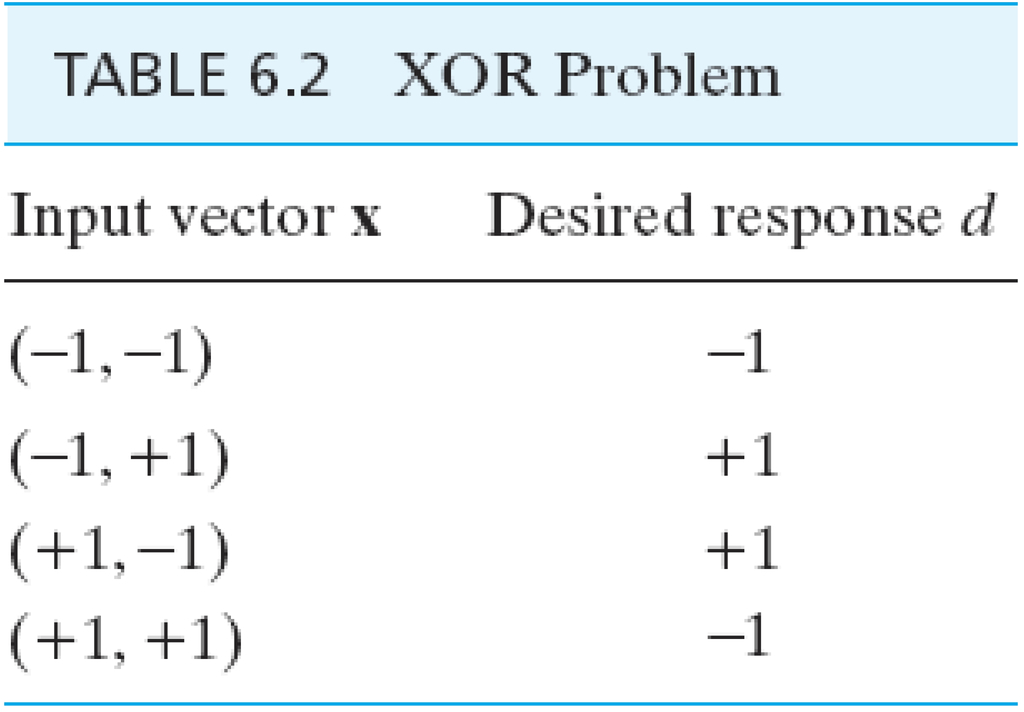
\includegraphics[width=0.5\linewidth]{fig10/lec1012.jpg}
\end{center}
\end{itemize}
\end{frame}


% 13
\begin{frame}[c]
\frametitle{XOR: first compute the kernel matrix}
\begin{itemize}
\item In general, $K_{ij}=k(\mathbf{x}_i,\mathbf{x}_j)=(1+\mathbf{x}_i^T\mathbf{x}_j)^2$
\item For example,

\[K_{11}=k
\begin{pmatrix}
\begin{bmatrix}
-1\\
-1\\
\end{bmatrix},\begin{bmatrix}
-1\\
-1\\
\end{bmatrix}
\end{pmatrix}=(1+2)^2=9
\]

\[K_{12}=k
\begin{pmatrix}
\begin{bmatrix}
-1\\
-1\\
\end{bmatrix},\begin{bmatrix}
-1\\
+1\\
\end{bmatrix}
\end{pmatrix}=(1+0)^2=1
\]
\item So

\[
K=
\begin{bmatrix}
9&1&1&1\\
1&9&1&1\\
1&1&9&1\\
1&1&1&9\\
\end{bmatrix}
\]
\end{itemize}
\end{frame}


% 14
\begin{frame}[c]
\frametitle{XOR: first compute the kernel matrix}
\begin{itemize}
\item Or compute $\phi(x_i)$ and their inner products, e.g.,
\begin{itemize}
\item $\phi(\mathbf{x})=[x_1^2,x_2^2,\sqrt2x_1x_2,\sqrt2x_1,\sqrt2x_2,1]$, where $1$ is added for $b$. 
\item Since $\phi (\mathbf{x})$ includes 1, no need for separate $b$ later

\[
\phi(\mathbf{x}_1)=\phi\begin{pmatrix}\begin{bmatrix}
-1\\
-1\\
\end{bmatrix}
\end{pmatrix}=
[1,1,\sqrt2,-\sqrt2,-\sqrt2,1]^T
\]

\[
\phi(\mathbf{x}_2)=\phi\begin{pmatrix}\begin{bmatrix}
-1\\
+1\\
\end{bmatrix}
\end{pmatrix}=
[1,1,-\sqrt2,-\sqrt2,\sqrt2,1]^T
\]
\end{itemize}
\item Then
\begin{gather*}
K_{11}=\phi^T(\mathbf{x}_1)\phi(\mathbf{x}_1)=1+1+2+2+2+1=9\\
K_{12}=\phi^T(\mathbf{x}_1)\phi(\mathbf{x}_1)=1+1-2+2-2+1=1
\end{gather*}
\item Results in same $K$ matrix, but more computation
\end{itemize}
\end{frame}




% 15
\begin{frame}[c]
\frametitle{XOR: Combine class labels into $K$}
\begin{itemize}
\item Define matrix $\tilde{K}$ such that $\tilde{K}_{ij}=K_{ij}d_id_j$
\item Recall $\mathbf{d}=[-1,+1,+1,-1]^T$
\[
\tilde{K}=
\begin{bmatrix}
+9&-1&-1&+1\\
-1&+9&+1&-1\\
-1&+1&+9&-1\\
+1&-1&-1&+9\\
\end{bmatrix}
\]
\end{itemize}
\end{frame}



% 16
\begin{frame}[c]
\frametitle{XOR: Solve dual Lagrangian for $a$}
\begin{itemize}
\item Find fixed points of
\[\tilde{L}(\mathbf{a})=\mathbf{1}^T\mathbf{a}-\dfrac{1}{2}\mathbf{a}^T\tilde{K}\mathbf{a}
\]
\item Set matrix gradient to 0
\begin{gather*}
\nabla \tilde{L}=\mathbf{1}-\tilde{K}\mathbf{a}=\mathbf{0}\\
\Rightarrow \mathbf{a}=\tilde{K}^{-1}\mathbf{1}=\begin{bmatrix}
\dfrac{1}{8},\dfrac{1}{8},\dfrac{1}{8},\dfrac{1}{8}
\end{bmatrix}^T
\end{gather*}
\item Satisfies all conditions: $a_p\geqslant{}0 \forall p$\qquad $\sum_pa_pd_p=0$
\begin{itemize}
\item So this is the solution
\end{itemize}
\item All points are support vectors
\end{itemize}
\end{frame}


% 17
\begin{frame}[c]
\frametitle{XOR: Compute $w$ (including $b$) from $a$}
\begin{gather*}
\mathbf{w}=\sum_pa_pd_p\mathbf{x}_p\\
=
-\dfrac18\phi(\mathbf{x}_1)
+\dfrac18\phi(\mathbf{x}_2)
+\dfrac18\phi(\mathbf{x}_3)
-\dfrac18\phi(\mathbf{x}_4)\\
=\dfrac{1}{8}
\begin{pmatrix}
-\begin{bmatrix}
1\\
1\\
\sqrt2\\
-\sqrt2\\
-\sqrt2\\
1\\
\end{bmatrix}
+\begin{bmatrix}
1\\
1\\
-\sqrt2\\
-\sqrt2\\
\sqrt2\\
1\\
\end{bmatrix}
+\begin{bmatrix}
1\\
1\\
-\sqrt2\\
\sqrt2\\
-\sqrt2\\
1\\
\end{bmatrix}
-\begin{bmatrix}
1\\
1\\
\sqrt2\\
\sqrt2\\
\sqrt2\\
1\\
\end{bmatrix}
\end{pmatrix}=
\begin{bmatrix}
0\\
0\\
-\dfrac{1}{\sqrt2}\\
0\\
0\\
0\\
\end{bmatrix}
\end{gather*}
\end{frame}




% 18
\begin{frame}[c]
\frametitle{XOR: Examine prediction function}
\begin{itemize}
\item Prediction function
\begin{gather*}
y(\mathbf{x})=\mathbf{w}^T\phi(\mathbf{x})\\
=\left[
0,
0,
-\dfrac1{\sqrt2}
0,
0,
0,\right]^T\left[
x_1^2,
x_2^2,
\sqrt2x_1x_2,
\sqrt2x_1,
\sqrt2x_2,
1\right]\\
=-x_1x_2
\end{gather*}

\item Predictions are based on product of the dimensions
\begin{gather*}
y(\mathbf{x}_1)=-(-1)(-1)=-1\\
y(\mathbf{x}_2)=-(-1)(+1)=+1\\
y(\mathbf{x}_3)=-(+1)(-1)=+1\\
y(\mathbf{x}_4)=-(+1)(+1)=-1
\end{gather*}
\end{itemize}
\end{frame}



% 19
\begin{frame}[c]
\frametitle{XOR: Decision boundaries}
\begin{itemize}
\item Decision boundary at $y(\mathbf{x})=-x_1x_2 = 0$
\item Support vectors at $y(\mathbf{x})=-x_1x_2 = 1$
\begin{center}
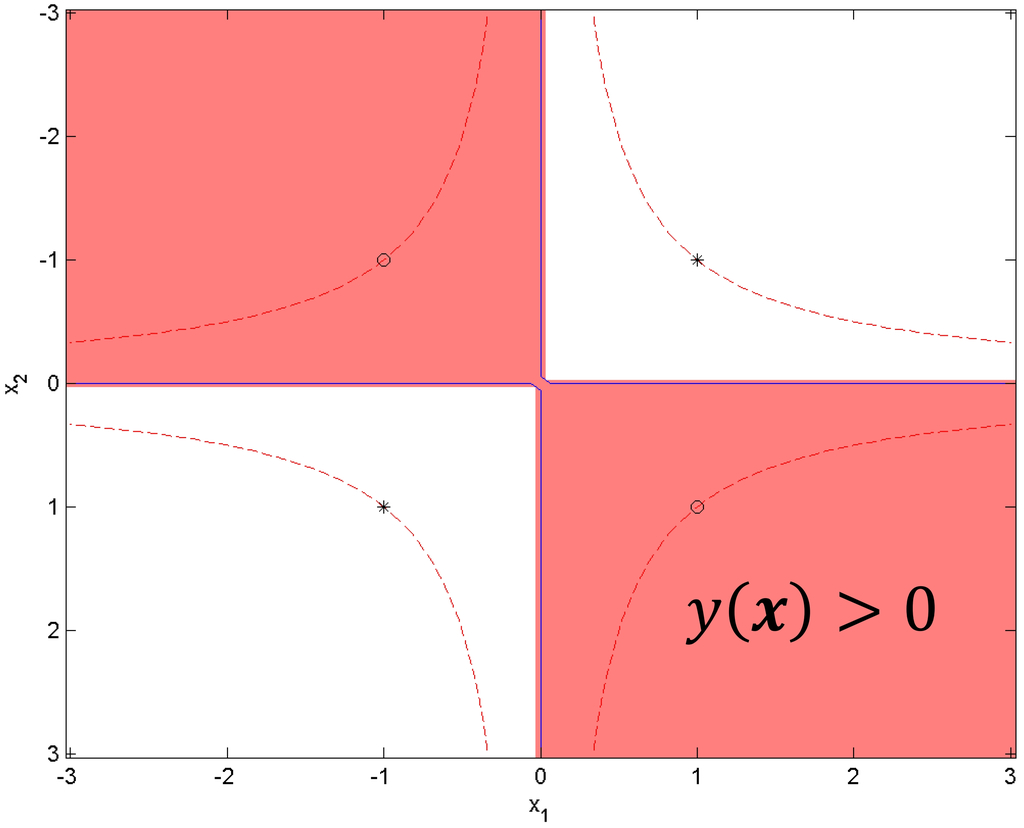
\includegraphics[width=0.7\linewidth]{fig10/lec1019.jpg}
\end{center}
\end{itemize}
\end{frame}




\begin{frame}
\begin{center}
\chuhao Thank you! %\fontspec{LHANDW.TTF}
\end{center}
\end{frame}
\end{document}
